\section{Diffusion Models}
\label{section:diffusion-models}

Diffusion models belong to the realm of probabilistic generative models, employing both forward and reverse probabilistic processes to transition between two distributions. These models are broadly classified into unconditional and conditional subclasses. In this section, we focus on Denoising Diffusion Probabilistic Models \cite{ho2020denoising} as an example of unconditional diffusion models, and Schrödinger Bridge as a representative of conditional diffusion models. Our aim is to explore the applications of SDEs in stochastic modeling, and establish the foundation for discussing the Image-to-image Schrödinger Bridge in the subsequent chapter on Related Works.

\subsection{Denoising Diffusion Probabilistic Models}
The idea of generating new samples in a distribution by firstly perturbs its sample to a known distribution (e.g. the Gaussian distribution) sparked from Score-based Generative Models (SGM) \cite{sohl2015deep}. DDPM progressed from SGM by using another forward and reverse strategy. Later, a continuous setting of DDPM using reverse SDEs was proposed \cite{song2020score}.

Firstly, let us explore the original strategy of DDPM. Let $\xbf_0$ be a random variable sampled from the dataset distribution $p_{\text{data}}$, and $\{\xbf_n\}_{n=1}^N$ be a Markov process, where $\xbf_n:\Omega\to\RR^d, n=1,\ldots,N$. Let $\{\beta_n\}_{n=1}^N\subset(0,1)$. The transition kernels are defined to be Gaussian
\begin{equation}
 q(\xbf_n|\xbf_{n-1})=\N(\xbf_n;\sqrt{1-\beta_n}\xbf_{n-1},\beta_n \mathbf{I}_d),\,\,\, i =1,\ldots,N.
\end{equation}
From these Gaussian transitions, we reformulate the sampling process as
\begin{equation}
 \label{equation:trans}
 \xbf_n = \sqrt{1-\beta_n}\xbf_{n-1}+\sqrt{\beta_n}\bm{\epsilon}_{n-1},
\end{equation}
where $\bm{\epsilon}_{n}\sim\N(\mathbf{0},\mathbf{I}_d), n=0,\ldots,N-1$. Note that two Gaussian distributed variables $\xbf\sim\N(\mathbf{0},\sigma_1^2\mathbf{I}_d)$ and $\mathbf{y}\sim\N(\mathbf{0},\sigma_2^2\mathbf{I}_d)$ have the sum
$\xbf+\mathbf{y}\sim \N(\mathbf{0},(\sigma_1^2+\sigma_2^2)\mathbf{I}_d)$. We have
\begin{align*}
 \xbf_1
  & = \sqrt{1-\beta_1}\xbf_{0}+\sqrt{\beta_1}\bm{\epsilon}_{0}                                                             \\
 \xbf_2
  & = \sqrt{1-\beta_2}\xbf_{1}+\sqrt{\beta_2}\bm{\epsilon}_{1}                                                             \\
  & =\sqrt{1-\beta_2}\left(\sqrt{1-\beta_1}\xbf_{0}+\sqrt{\beta_1}\bm{\epsilon}_{0}\right)+\sqrt{\beta_2}\bm{\epsilon}_{1} \\
  & =\sqrt{(1-\beta_1)(1-\beta_2)}\xbf_{0}+\sqrt{(1-\beta_2)\beta_1+\beta_2}\Tilde{\bm{\epsilon}}_{2}                      \\
  & =\sqrt{(1-\beta_1)(1-\beta_2)}\xbf_{0}+\sqrt{1-(1-\beta_1)(1-\beta_2)}\Tilde{\bm{\epsilon}}_{2},
\end{align*}
where $\Tilde{\bm{\epsilon}}_{2}\sim\N(\mathbf{0},\mathbf{I}_d)$. Consequently, let $\alpha_n=\prod\limits_{m=1}^i(1-\beta_m)\in (0,1), 0\le n \le N-1$. We have
\begin{equation}
 \xbf_n = \sqrt{\alpha_n}\xbf_0 + \sqrt{1- \alpha_n}\Tilde{\bm{\epsilon}}_{i}\sim\N(\sqrt{\alpha_n}\xbf_0, (1- \alpha_n)\mathbf{I}_d)
\end{equation}
Since $\alpha_N$ is the product of $N$ elements less than one, when $N$ is large, $\sqrt{\alpha_N}\to 0$ and $1-\alpha_N\to 1$. Hence, $\xbf_N\sim \N(\mathbf{0},I_d)$. This is the reason we choose the standard Gaussian at the beginning of our reverse process. Due to the Markov property
\begin{align*}
 q(\xbf_0,\xbf_1,\xbf_2)
  & = q(\xbf_0,\xbf_1)q(\xbf_2|\xbf_0,\xbf_1)                   \\
  & =q(\xbf_0)q(\xbf_1|\xbf_0)q(\xbf_2|\xbf_1)                  \\
 q(\xbf_0,\xbf_1,\xbf_2,\xbf_3)
  & = q(\xbf_0,\xbf_1,\xbf_2)q(\xbf_3|\xbf_0,\xbf_1,\xbf_2)     \\
  & =q(\xbf_0)q(\xbf_1|\xbf_0)q(\xbf_2|\xbf_1)q(\xbf_3|\xbf_2).
\end{align*}
Consequently,
\begin{equation} q(\xbf_0,\ldots,\xbf_N)=q(\xbf_0)\prod\limits_{i=1}^Nq(\xbf_i|\xbf_{i-1}).
\end{equation}

\begin{table}[H]
 \begin{center}
  \begin{tabular}{cc}
   \hline
   \textbf{}  & \textbf{Setting}                                              \\ \hline
   ODE solver & Euler                                                         \\
   Time steps & $1 + \frac{i}{N+1}(\epsilon_s -1)$                            \\
   Schedule   & $\sigma = \sqrt{e^{\frac{1}{2}\beta_d t^2 + \beta_{min}t}-1}$ \\
   Scaling    & $\alpha = 1/\sqrt{e^{\frac{1}{2}\beta_d t^2 + \beta_{min}t}}$ \\ \hline
   Parameters & $\beta_d = 19.9, \beta_{min} = 0.1$                           \\
              & $\epsilon_s = 10^{-3}, \epsilon_t = 10^{-5}$                  \\
              & $M = 1000$                                                    \\ \hline
  \end{tabular}
 \end{center}
 \caption{Simulation setting for DDPM forward process}
 \label{table:simulation-setting-for-forward-ddpm}
\end{table}

We construct the forward process for an image with parameters given in Table \ref{table:simulation-setting-for-forward-ddpm}, the result is also used for diffusion illustration in Figure \ref{figure:diffusion-illustration}. To check whether the final image is Gaussian, we visualized in Figure \ref{figure:Histogram} a weaker condition - the histograms on values from $0$ to $255$ for each channel of the image at timesteps $0$, $1$, and $1000$. The histogram represents the distribution of pixel values for each channel namely, red, green, and blue. The visualizations are presented. By the last step, timestep 1000, the histograms for all three channels have transformed into a complete Gaussian distribution pattern. This transformation suggests that the forward process gradually shifts the data distribution towards a Gaussian pattern.

\begin{figure}[H]
 \centering
 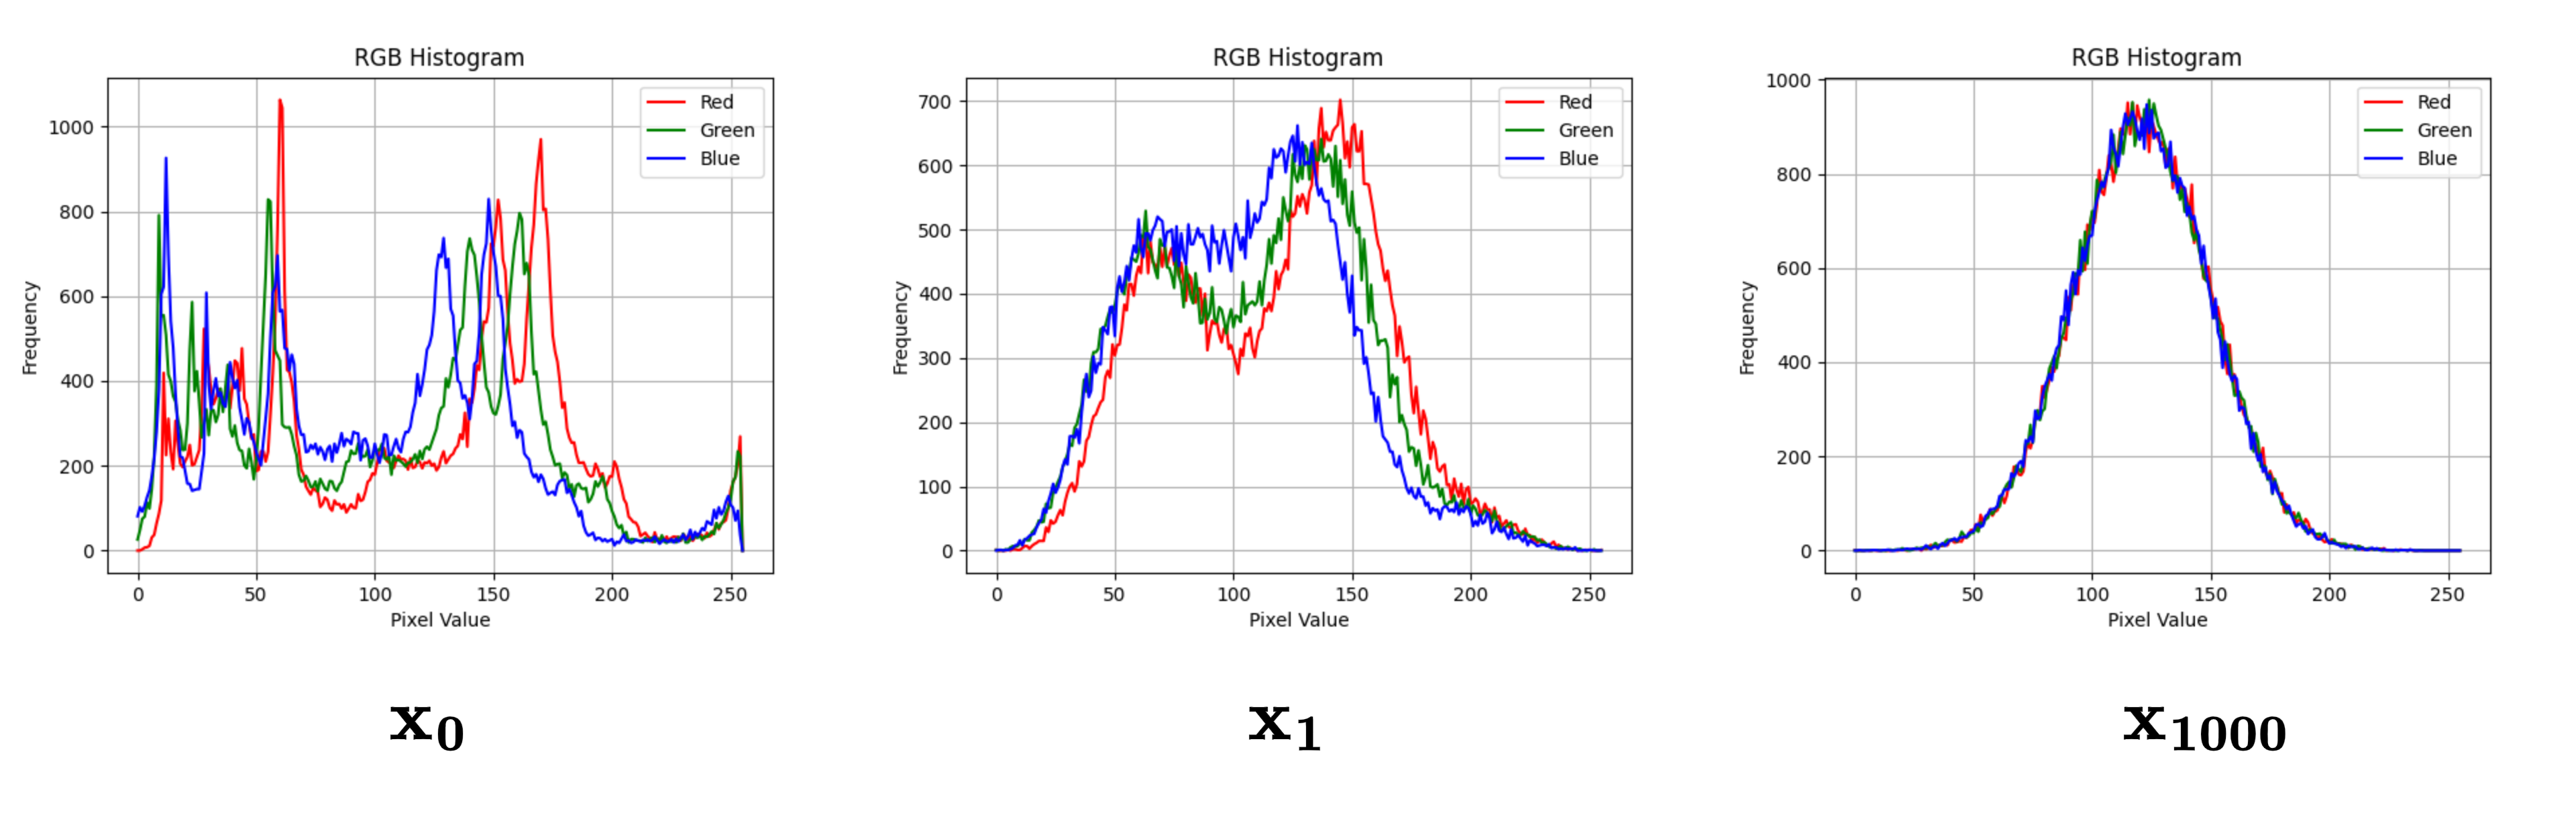
\includegraphics[width = \textwidth]{img/Histogram.png}
 \vspace{0.1cm}
 \caption{Histogram visualization for the forward process}
 \label{figure:Histogram}
\end{figure}

The ennoising process converted a data sample to a normal-distributed sample. Now we establish a process denoises a normal-distributed sample to a sample approximated to a data distribution. The reason is that we can minimize each sample during the ennoising and denoising processes to derive a suitable denoising process. Starting from the standard Gaussian noise $\overline{\xbf}_N\sim p_\theta(\overline{\xbf}_0):=\N(\mathbf{0},I_d)$, we need a decent way of performing denoising to retrieve $p_\text{data}$. Here we parameterize the reverse transitions by an U-Net \cite{ho2020denoising} as Gaussian distributions
\begin{equation}
 \label{equation:ddpm_reveverse}
 p_\theta(\overline{\xbf}_{n-1}|\overline{\xbf}_{n})=\N(\overline{\xbf}_n;\bm{\mu}(\overline{\xbf}_{n},i),\bm{\Sigma}(\overline{\xbf}_{n},i)), n=1,\ldots,N
\end{equation}
which constitutes the reverse joint probability density
\begin{equation}
 p_\theta(\overline{\xbf}_0,\ldots,\overline{\xbf}_N)=p_\theta(\overline{\xbf}_0)\prod\limits_{n=1}^Np_\theta(\Tilde{\xbf}_n|\overline{\xbf}_{n-1}).
\end{equation}
We would like to train the model so that we can generate samples via the reverse Markov processes, i.e. $p_\theta(\overline{\xbf}_0)\approx p_{\text{data}}(\xbf_0):=q(\xbf_0)$. An
apparent estimation of the parameter $\theta$ is that the forward and reverse states coincide correspondingly, i.e. $\xbf_n\approx\overline{\xbf}_{n}$, for $n=1,\ldots,N$ and $\xbf_N\approx\overline{\xbf}_{0}\sim\N(\mathbf{0},\mathbf{I}_d)$. As such, we should
expect the joint density with respect to the forward and the reverse processes are equal, i.e.
$$p_\theta(\overline{\xbf}_0,\ldots,\overline{\xbf}_N)\simeq q(\xbf_0,\ldots,\xbf_N).$$

Therefore, we can minimize the Kullback-Leibler divergence (see Equation \ref{definition:KL-divergence}) from $q(\xbf_0,\ldots,\xbf_N)$ to $p_\theta(\overline{\xbf}_0,\ldots,\overline{\xbf}_N)$.
\begin{equation}
 \label{equation:KL-yang}
 D_{\text{KL}}(q(\xbf_0,\ldots,\xbf_N)\| p_\theta(\overline{\xbf}_0,\ldots,\overline{\xbf}_N)) = \EE_{q(\xbf_0,\ldots,\xbf_N)}\left[\dfrac{q(\xbf_0,\ldots,\xbf_N)}{p_\theta(\overline{\xbf}_0,\ldots,\overline{\xbf}_N)}\right].
\end{equation}

\begin{figure}[H]
 \centering
 \scalebox{0.8}{
  \begin{tikzpicture}[->,>=stealth,shorten >=1pt,auto,node distance=2.3cm,semithick]
   % Forward process
   \node[state,minimum size=1.2cm] (A)  {$\xbf_0$};
   \node[state,minimum size=1.2cm,fill=lightgray] (B) [right of=A] {$\xbf_1$};
   \node[state,minimum size=1.2cm,fill=lightgray] (C) [right of=B] {$\xbf_2$};
   \node        (D) [right of=C] {$\cdots$};
   \node[state,minimum size=1.2cm,fill=lightgray] (E) [right of=D] {$\xbf_{N-2}$};
   \node[state,minimum size=1.2cm,fill=lightgray](F) [right of=E] {$\xbf_{N-1}$};
   \node[state,minimum size=1.2cm,fill=lightgray] (G) [right of=F] {$\xbf_N$};

   \path (A) edge              node {} (B)
   (B) edge              node {} (C)
   (C) edge              node {} (D)
   (D) edge              node {} (E)
   (E) edge              node {} (F)
   (F) edge              node {} (G);

   \node (image) [below of=D]{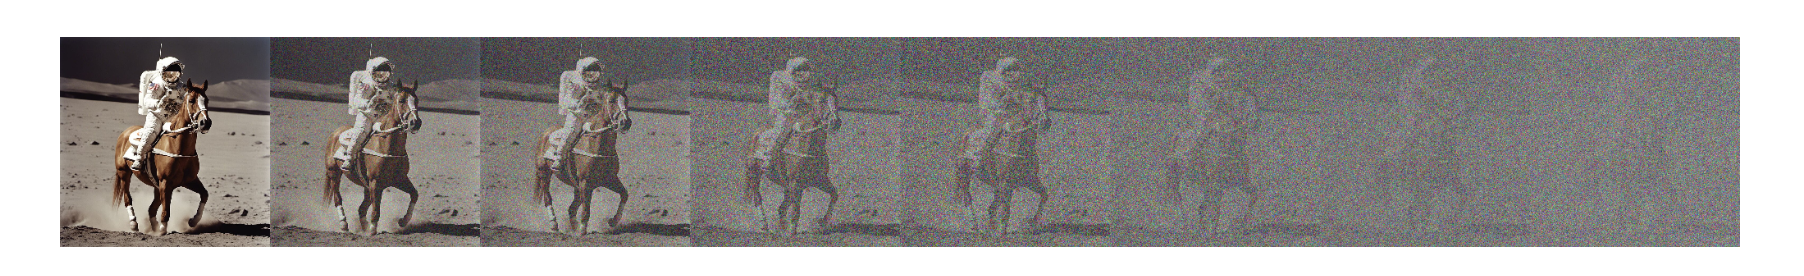
\includegraphics[width=\textwidth]{img/diffusion-illustration.png}};

   % Reverse process
   \node        (K) [below of=image] {$\cdots$};
   \node[state,minimum size=1.2cm,fill=lightgray] (J) [left of=K] {$\overline{\xbf}_{2}$};
   \node[state,minimum size=1.2cm,fill=lightgray] (I) [left of=J] {$\overline{\xbf}_{1}$};
   \node[state,minimum size=1.2cm] (H) [left of=I] {$\overline{\xbf}_N$};
   \node[state,minimum size=1.2cm,fill=lightgray] (L) [right of=K] {$\overline{\xbf}_{N-2}$};
   \node[state,minimum size=1.2cm,fill=lightgray] (M) [right of=L] {$\overline{\xbf}_{N-1}$};
   \node[state,minimum size=1.2cm,fill=lightgray](N) [right of=M] {$\overline{\xbf}_0$};

   \path (I) edge              node {} (H)
   (J) edge              node {} (I)
   (K) edge              node {} (J)
   (L) edge              node {} (K)
   (M) edge              node {} (L)
   (N) edge              node {} (M);
  \end{tikzpicture}
 }
 \caption[An illustration of DDPMs by Markov processes.]{An illustration of DDPMs by Markov processes. }
 \label{figure:diffusion-illustration}
\end{figure}

Now we will see how SDEs are applied, by using arbitrary intermediate time points. Let $\{\beta_t\}_{t\ge0}$ be the set of scheduled noise variance.
Let $\Delta t>0$ be an arbitrary time step. We follow Song et al. \cite{song2020score} to define $\beta(t)=\dfrac{\beta_t}{\Delta t_0}$ and thus
\begin{align*}
 \xbf_{t+\Delta t}-\xbf_{t}
  & = (\sqrt{1-\beta_t\Delta t}-1)\xbf_{t}+\sqrt{\beta_t}\sqrt{\Delta t}\bm{\epsilon}_{t}       \\
  & =(\sqrt{1-\beta_t\Delta t}-1)\xbf_{t}+\sqrt{\beta_t}(\mathbf{W}(t+\Delta t)-\mathbf{W}(t)).
\end{align*}

As $\Delta t\to 0$, we use an approximation
\begin{equation}
 \sqrt{1-\beta(t)\Delta t} - 1\approx -\dfrac{1}{2}\beta(t)\Delta t
\end{equation}
to arrive at a forward SDE
\begin{equation}
 \label{equation:song-sde}
 \d \xbf(t)=-\dfrac{1}{2}\beta(t)\xbf(t)\d t+\sqrt{\beta(t)}\d \mathbf{W}(t).
\end{equation}
Using Theorem \ref{theorem:reverse-time-sde}, the corresponding reverse-time SDE is
\begin{equation}
 \d \xbf_t = \left[-\dfrac{1}{2}\beta_t \xbf_t-\beta_t\nabla_{\xbf_t}\log p(\xbf_t, t)\right]\d t + \beta(t)\d \mathbf{W}_t.
\end{equation}
Therefore, using forward-backward SDEs, we only have to approximate $\nabla_{\xbf_t}\log p(\xbf_t, t)$, called the score function of $X_t$ i.e. to train a score network
$$\mathbf{s}_\theta(\xbf,t) \approx \nabla_{\xbf_t}\log p_t(\xbf_t)$$
instead of a network to approximate $\bm{\mu}(\overline{\xbf}_{n},i)$ and $\bm{\Sigma}(\overline{\xbf}_{n},i)$.

\subsection{Schrödinger Bridge}
Whereas unconditional diffusion models generate new samples in the dataset distribution, conditional diffusion models transform a sample from an initial distribution $p_{\A}$ to a target distribution $p_{\B}$. Schrödinger Bridge (SB) is an entropy-regularized optimal transport model that considers the following forward and backward SDEs \cite{schrodinger1932theorie}. In this discussion of SB, let us simplify the diffusion time interval to $[0,1]$. The forward-reverse SDEs in SB is given by
\begin{align}
 \label{equation:sb-fw}
 \d\xbf_t & = [\mathbf{f}_t + \beta_t\nabla\log\Psi(\xbf_t,t)]\d t + \sqrt{\beta_t}\d \mathbf{W}_t,           & \,\,\, \xbf_0\sim p_{\A}  \\
 \label{equation:sb-bw}
 \d\xbf_t & = [\mathbf{f}_t - \beta_t\nabla\log\hat{\Psi}(\xbf_t,t)]\d t-\sqrt{\beta_t}\d \bar{\mathbf{W}}_t, & \,\,\, \xbf_1\sim p_{\B}.
\end{align}

\begin{theorem}
 If $\Psi,\hat{\Psi}\in C^2(\RR^d,[0,1])$ satisfying
 \begin{equation}
  \label{equation:sb-condition}
  \begin{cases}
   \dfrac{\partial\Psi(\xbf,t)}{\partial t} = -\nabla \Psi^\top f-\dfrac{1}{2}\beta\Delta\Psi                      \\
   \dfrac{\partial\hat{\Psi}(\xbf,t)}{\partial t} = -\mathrm{div} (\hat{\Psi} f)+\dfrac{1}{2}\beta\Delta\hat{\Psi} \\
  \end{cases}
 \end{equation}
 The boundary conditions are $\Psi(x,0)\hat{\Psi}(x,0)=p(x,0)$ and $\Psi(x,1)\hat{\Psi}(x,1)=p(x,1)$.
 Then (\ref{equation:sb-bw}) is the reverse-time SDE of (\ref{equation:sb-fw}).
\end{theorem}
\begin{proof}
 The condition (\ref{equation:sb-condition}) suggests Nelson duality between $\Psi$ and $\hat{\Psi}$ \cite{nelson2020dynamical}
 $$\Psi(x,t)\hat{\Psi}(x,t)=p(x,t).$$
 Hence,
 $$\log\nabla\Psi(x,t) + \log\nabla\hat{\Psi}(x,t)=\log\nabla p(x,t).$$
 According to Theorem \ref{theorem:reverse-time-sde}, the reverse-time SDE of (\ref{equation:sb-fw}) is
 \begin{align*}
  \d X_t
   & = [f_t + \beta_t\nabla\log \Psi - \beta\nabla\log p(x,t)]\d t + \sqrt{\beta}\d W                             \\
   & = [\mathbf{f}_t - \beta_t\nabla\log\hat{\Psi}(\xbf_t,t)]\d t-\sqrt{\beta_t}\d \bar{\mathbf{W}}_t.
 \end{align*}
\end{proof}

\begin{theorem}
 Let (\ref{equation:sb-fw}) and (\ref{equation:sb-bw}) be a pair of forward-reverse SDEs. Then $\nabla\log\hat{\Psi}(x,t)$ and $\nabla\log{\Psi}(x,t)$ are the score functions of the following SDEs, respectively
 \begin{align}
  \label{equation:sde-psihat}
  \d X_t & = f_t\d t + \sqrt{\beta_t} \d W, & X_0\sim \nabla\log\hat{\Psi}(x,0) \\
  \label{equation:sde-psi}
  \d X_t & = f_t\d t + \sqrt{\beta_t} \d W, & X_0\sim \nabla\log{\Psi}(x,1).
 \end{align}
\end{theorem}
\begin{proof}
 Write the forward Kolmogorov equations and substitute conditions (\ref{equation:sb-condition}) to yield the results.
\end{proof}